

\section{Inter-Layer Prediction in SVC}
\label{sec:inter-layer-prediction}

    The purpose of inter-layer prediction in Scalable Video Coding (SVC) is to
    reduce the redundancy between the base layer and enhancement
    layers. This allows for higher compression efficiency without significantly
    increasing decoder complexity. These prediction tools are inspired by
    traditional single-layer prediction techniques in H.264/AVC but are extended
    to operate across layers.

    In H.264/AVC, each macroblock is coded using either intra (texture) or inter (motion)
    prediction:

    \begin{itemize}
        \item 
            \textbf{Texture prediction:} 
            Uses spatial correlation by predicting the current MB from
            neighboring MBs within the same picture.

        \item 
            \textbf{Motion prediction:} 
            Uses temporal correlation by referencing previously decoded frames.
            Motion vectors and reference indices are used to point to predictive
            blocks in reference pictures.

        \item 
            \textbf{Residual prediction:} 
            After prediction (intra or inter), the difference/residual between the
            original and predicted block is transformed,
            quantized, and coded.
    \end{itemize}

    In SVC, these same principles are extended across layers through inter-layer
    prediction, where the enhancement layer reuses information from the
    co-located MB in the base layer:

    \begin{itemize}
        \item 
            \textbf{Inter Layer Texture Prediction:} 
            Analogous to intra prediction, but instead of spatial neighbors, the
            enhancement layer MB uses the reconstructed and upsampled co-located
            MB from the base layer. This enables the MB to be coded as
            \textit{IntraBL}, saving bits by avoiding spatial prediction and
            residual transmission.

        \item 
            \textbf{Inter Layer Motion Prediction:} 
            Similar to AVC inter prediction, but the motion vectors, reference
            indices, and partitioning of the base layer MB are reused in the
            enhancement layer. For dyadic spatial scalability, motion vectors
            are upsampled by a factor of 2. Quarter-pel refinement can
            optionally be applied to improve precision.

        \item 
            \textbf{Inter Layer Residual Prediction:} 
            While AVC encodes the residual directly, SVC enhances this by
            allowing the residual of the base layer MB to be upsampled and
            subtracted from the enhancement layer residual before encoding. The
            encoder then transmits only the difference, reducing the residual
            bitrate.

    \end{itemize}

    Rate-Distortion Optimization (RDO) is used to decide whether to use these
    inter-layer modes on a per-macroblock basis, balancing bit cost against
    prediction accuracy.


\section{Macroblock Skips and Virtual Quality Levels}
\label{sec:virtual_quality_levels}
    In this section, we investigate whether intermediate quality levels beyond
    the explicitly defined scalability layers can be created by partially
    omitting enhancement-layer data.

    As introduced in Section~\ref{sec:svc-bitstream-structure}, the SVC
    bitstream is composed of access units, each containing slices corresponding
    to different enhancement layers. Each slice includes a slice header and a
    slice data section, which holds a list of macroblocks. Macroblocks are the
    smallest coding units in the video and contain motion, prediction, and
    residual data used by the decoder to reconstruct the frame.

    The slice data structure in the scalable extension is defined by the syntax
    shown in  Figure~\ref{fig:slice-data-syntax}.  A key element of this syntax
    is the \texttt{mb\_skip\_flag}, which indicates whether a macroblock is
    skipped. Macroblocks can be skipped when their content can be
    predicted from reference frames with minimal impact on visual
    quality The primary purpose of macroblock skip mode in the H.264 is to
    reduce bitrate by avoiding the transmission of redundant information.  When
    this flag is set, no motion vectors or residuals are transmitted for that
    macroblock and corresponding
    \texttt{macroblock\_layer\_in\_scalable\_extension()} syntax is omitted from
    the bitstream. Instead, the decoder reconstructs it using motion-compensated
    prediction from a reference frame. This mechanism is highly efficient, often
    requiring only a single bit to encode the skip decision, resulting in a
    reduced bitrate with minimal perceptual impact.


    This skipping mechanism applies only to macroblocks in P and B-macroblocks, which
    are inter-coded and can be predicted using motion information and residuals
    from reference frames. In contrast, intra-coded I-macroblocks rely
    entirely on spatial prediction within the same frame and do not use motion
    vectors or residuals from other frames. Since there is no external reference
    available, skipping intra-coded macroblocks is not possible, and they must
    always be fully encoded.

    \begin{figure}[H]
        \centering
        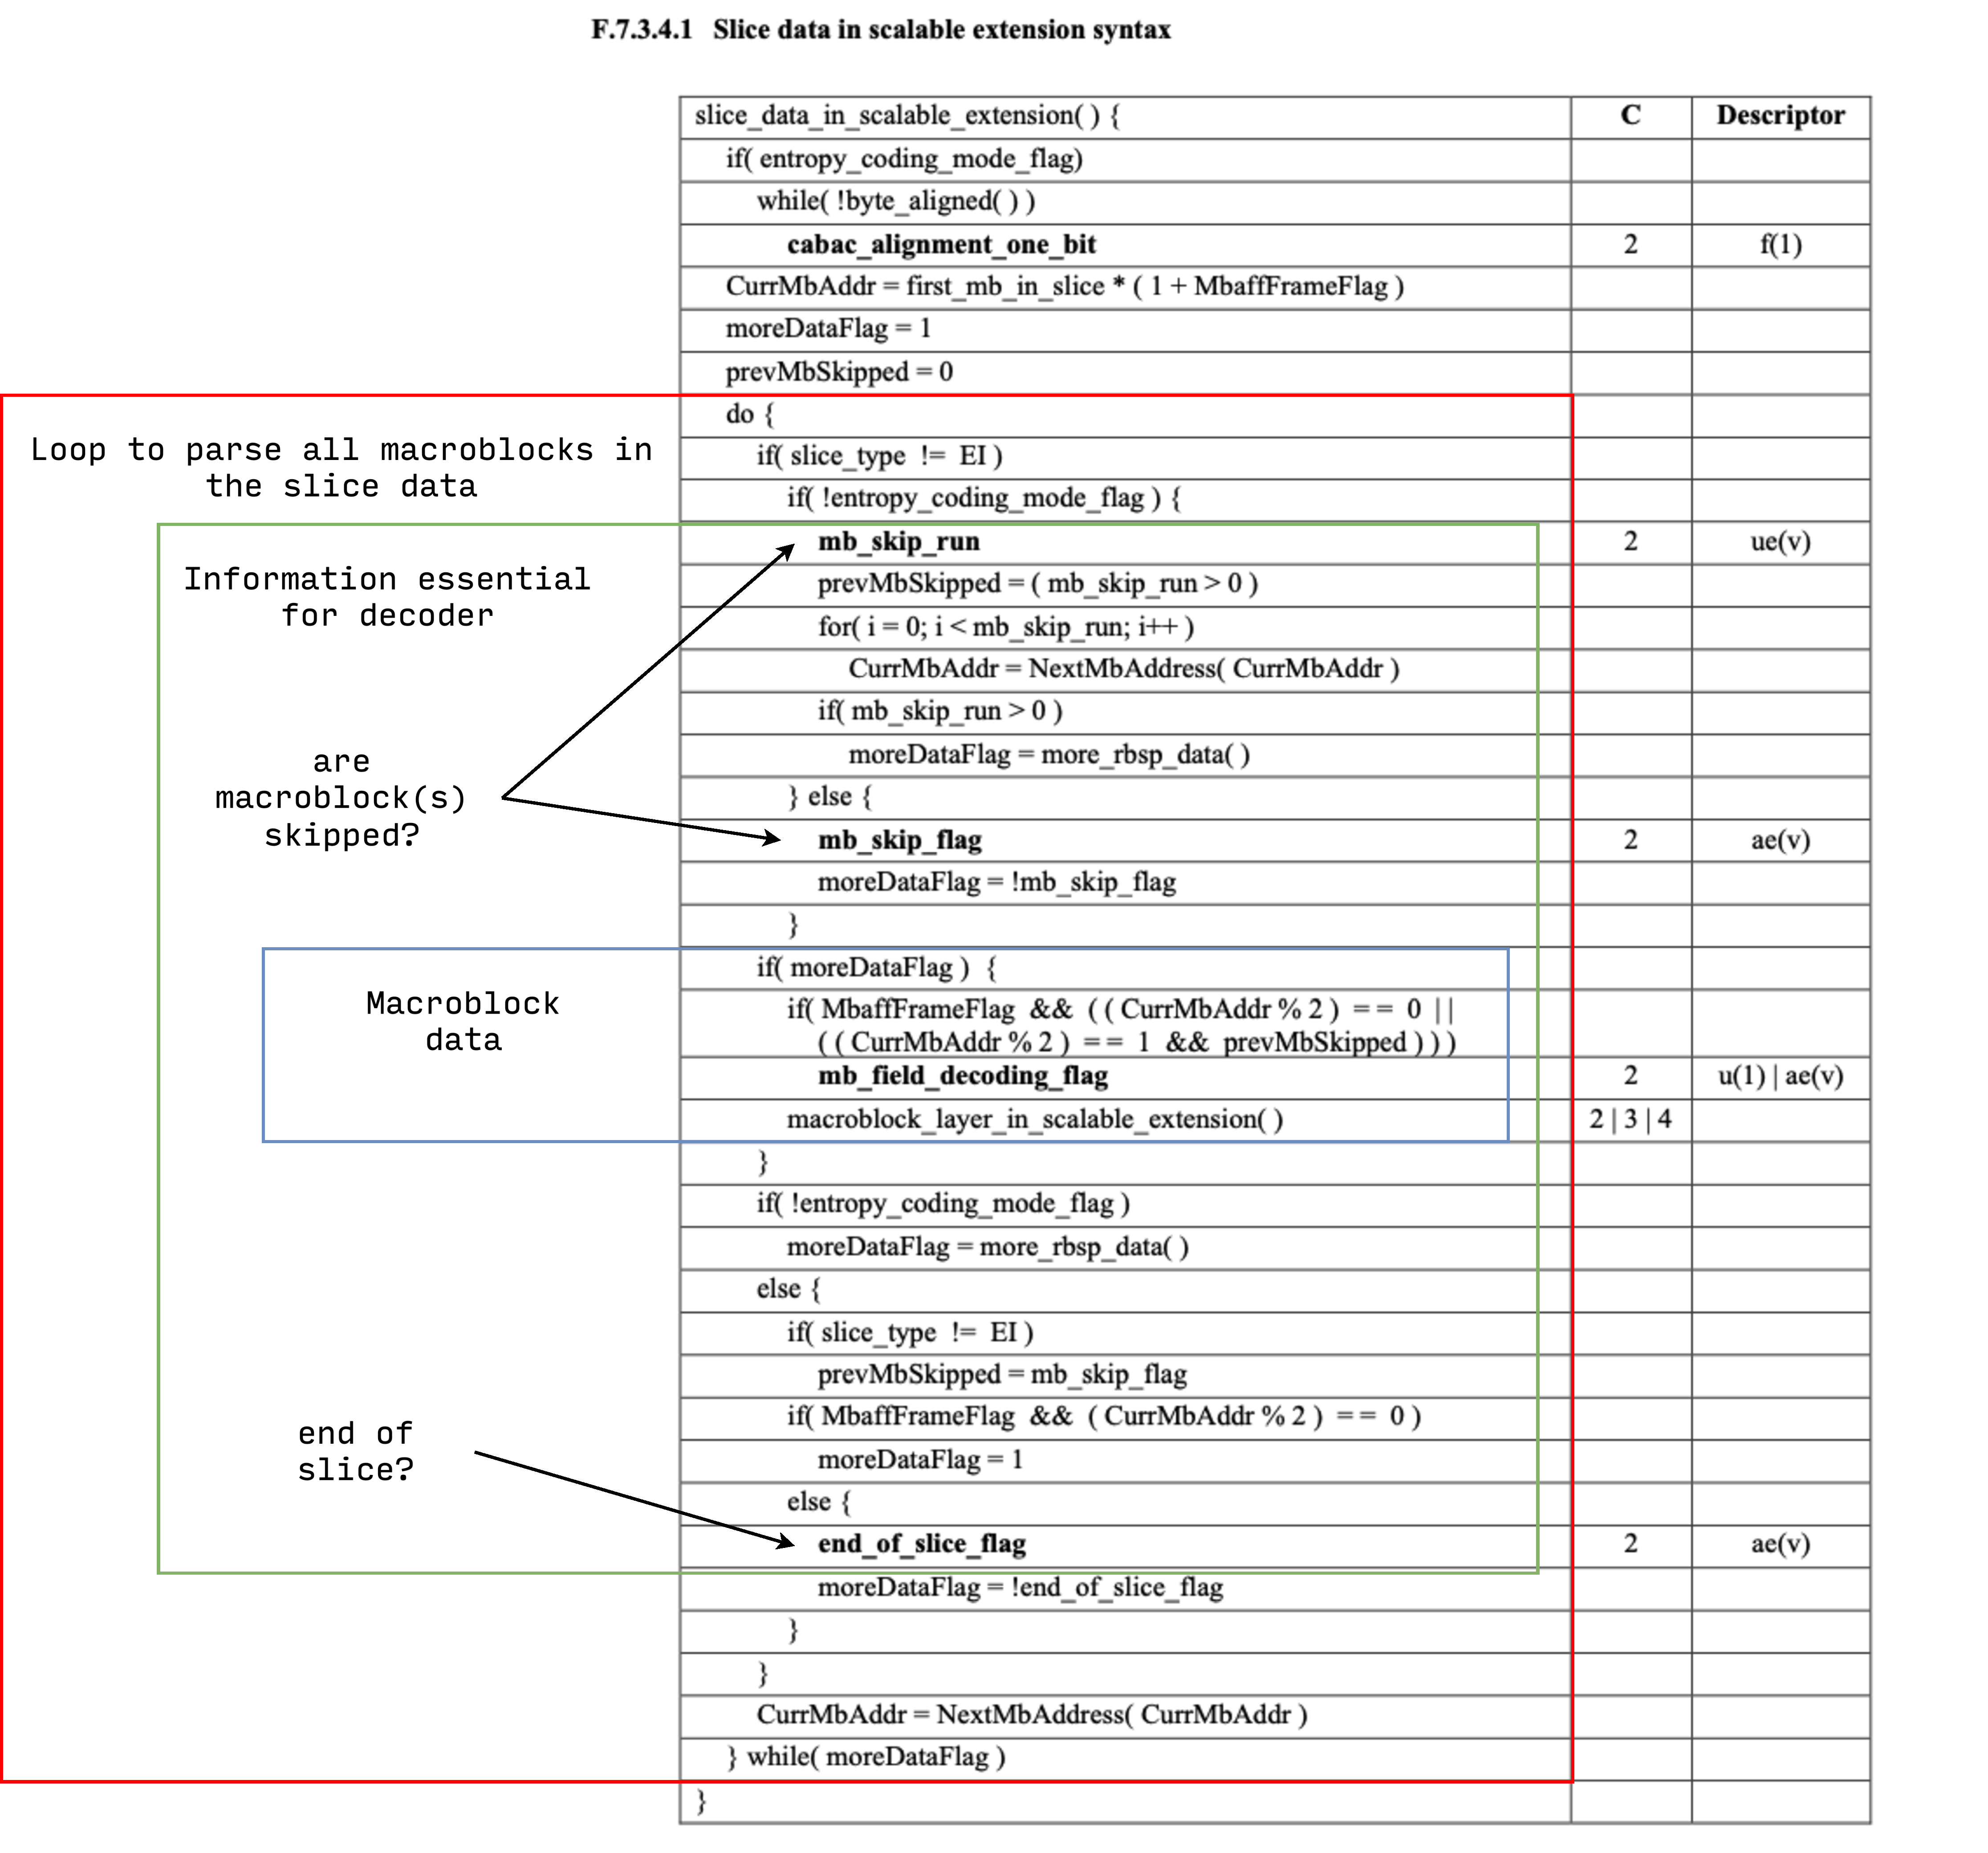
\includegraphics[width=\linewidth]{slice-data-syntax.pdf} 
        \caption{Slice data syntax in H.264/SVC}
        \label{fig:slice-data-syntax}
    \end{figure}

    In our approach, we leverage this skip mechanism to omit
    macroblocks in the enhancement layers. For each macroblock we want to skip,
    we set the \texttt{mb\_skip\_flag} and remove the associated
    \texttt{macroblock\_layer\_in\_scalable\_extension()} syntax. This allows us
    to drop enhancement layer data in a controlled way while preserving
    the decodability of the bitstream.
    

    By skipping macroblocks in the enhancement layers, we create
    modified versions of the original bitstream that has degraded visual quality.
    These degraded versions represent
    quality levels that are not explicitly provided by the original SVC bitstream.
    We refer to these intermediate representations as \textit{virtual quality
    levels}. Each virtual level reflects a unique quality point created by partially
    omitting enhancement data, offering finer granularity between the standard
    quality steps defined by the encoder. This allows for smoother quality
    transitions and more flexible adaptation to available network resources than
    conventional SVC layer switching.


    In the following sections, we evaluate these virtual quality levels using
    objective video quality metrics such as SSIM, PSNR, and VMAF, and assess
    their potential for improving streaming adaptability under fluctuating
    network conditions.


\section{Motion and Residual Upsampling}
\label{sec:blskip}
    Macroblock skips can produce unacceptable playback quality due to missing
    data.  In order to prevent such effects, error concealment techniques are
    highly desirable.

    Error concealment refers to the techniques used to recover missing or
    corrupted data, typically due to packet losses during transmission. SVC error concealment techniques
    rely on spatial, temporal, or inter-layer redundancy to estimate the
    lost information and maintain acceptable playback quality. While originally
    designed to address unintentional losses, such techniques are also effective in
    scenarios involving deliberate omission of data.

    In our approach, we use the \textit{Base Layer Skip (BLSkip)} error
    concealment method to reconstruct macroblocks that are skipped in
    the enhancement layer. For skipped macroblocks in the enhancement layer, BLSkip
    operates as follows:
    
    \begin{enumerate}
        \item 
        If the co-located macroblock in the base layer is
        intra-coded, inter-layer texture prediction is used to generate the enhancement
        layer content. 
        
        \item
        If the co-located macroblock in the base layer is inter-coded, both inter-layer
        motion prediction and residual prediction are applied. In this case, motion
        compensation is performed in the enhancement layer using the upsampled
        motion vectors from the base layer, and the residual signal is predicted
        accordingly. 
    \end{enumerate}
    
    This enables reconstruction of the skipped macroblock while preserving visual quality.


